\documentclass[12pt,a4paper]{book}

\setcounter{tocdepth}{3}

\usepackage[utf8]{inputenc}
\usepackage[french]{babel}
\usepackage[T1]{fontenc}
\usepackage{graphicx}
\usepackage{fullpage}
\usepackage{url}
\usepackage{caption}
\usepackage{subcaption}

\usepackage{amsmath}
\usepackage{amsfonts}
\usepackage{dsfont}
\usepackage{amssymb}

\usepackage{comment}

\usepackage{amsthm}
\newtheorem{env_definition}{Définition}
\newtheorem{formule}{Formule}
\newtheorem{annexe}{Annexe}

\usepackage[colored]{shadethm}
\definecolor{shadethmcolor}{rgb}{1,0.871,0.890}% couleur du fond
\definecolor{shaderulecolor}{rgb}{0.651,0.074,0.090}% couleur de l'encadré
\newshadetheorem{env_proposition}{Proposition}
\newshadetheorem{env_lemme}{Lemme}
\newshadetheorem{theorem}{Théorème}

\newcommand{\R}{\mathbb{R}}

\renewcommand\thesection{\Roman{section}}

\newcommand{\E}{\mathbb{E}}
\newcommand{\p}{\mathbb{P}}
\newcommand{\1}{\mathds{1}}

\DeclareMathOperator*{\argmin}{arg\!\min}


\usepackage{pythonhighlight}
%\usepackage[margin=0.5in]{geometry}
\usepackage{color, colortbl}
\usepackage{xcolor}
\usepackage{graphicx}
\usepackage{caption}


\definecolor{Gray}{gray}{0.9}
\definecolor{DarkGray}{gray}{0.5}
\definecolor{LightCyan}{rgb}{0.88,1,1}
\definecolor{yellow}{rgb}{1,1,0}

\begin{document}



% Page de garde
	
\begin{titlepage}
	\thispagestyle{empty}
	\begin{center}
	
    
\includegraphics[scale=1.]{Logo}  
	\vspace{1 cm}

	
	\vspace{0.7 cm}
	\textbf{{\fontsize{26}{34} \selectfont Prédiction de la Production de Bière en Australie }}\\
	\vspace{1 cm}
	 
	
	\vspace{1.5 cm}
	{\fontsize{15}{25} \selectfont Par : \\
		\item Philippine RENAUDIN
		\item Elvina EURY
	}\\
	\vspace{0.5 cm}
	{\fontsize{15}{25} \selectfont Master 2 Mathématiques et Applications}\\
	{\fontsize{15}{25} \selectfont Parcours Data Science}\\
	\vspace{1 cm}
	{\fontsize{10}{25} \selectfont Sous la direction de M. Frédéric Proia}
	\vspace{1.5 cm}

	{\fontsize{20}{30} \selectfont 2020-2021}\\
	
	\end{center}
\end{titlepage}

\thispagestyle{empty}
\newpage


% Table des matières


% Description du sujet

\newpage
\setcounter{page}{1}

\noindent
{\LARGE \textbf{Introduction}}
\vspace{5 mm}

%===============================================================================

	Dans le cadre de cette étude nous disposons de données de production mensuelle de bière en Australie (en megalitre), de janvier 1956 à août 1995. L'objectif est de prédire la production de bière pour les trois années suivantes, c'est-à-dire du mois de septembre 1995 au mois de septembre 1998, en modélisant les données à l'aide de séries chronologiques.
Dans un premier temps, nous analysons les données afin de déterminer une présence ou absence de tendance et de périodicité. Ensuite nous mettons en place plusieurs modèles qui nous semblent pertinents, et ce en se basant sur différentes caractéristiques des données. Enfin, nous comparons les performances de nos modèles sur un critère prédictif et ne gardons que les deux meilleurs. A partir de ces deux modèles, nous prédisons donc les valeurs pour les 36 mois suivants.

\vspace{5 mm}

%===============================================================================

\noindent
\section{Analyse des données et premières visualisations}

\subsection{Visualisation des données}

La modélisation par séries chronologiques peut s'écrire comme suit :\\ 
$X_t = m_t + S_t + Z_t $
où $X_t$ est la valeur de la série à l'instant t.


$m_t$ est la tendance et représente l'évolution de la série sur le long terme.
$S_t$ est la saisonnalité et représente l'évolution à court terme de la série. La saisonnalité traduit l'éventuelle périodicité des données.
$Z_t$ est la partie non déterministe du processus et est donc qualifié de fluctuations. C'est le reste de l'information non expliquée par la tendance ou la saisonnalité.
L'écriture de $X_t$ ci dessus suppose que le modèle est additif. Or, il est tout à fait possible qu'il y ait des phénomènes d'amplification, auquel cas un modèle additif n'est pas adapté. On lui préférera un modèle multiplicatif de la forme : $X_t = m_t*S_t*Z_t$.

\vspace{10 mm}
La Figure 1 représente la série (à gauche) et le logarithme de la série (à droite). \\
Une première observation visuelle de la série met en évidence une tendance (linéaire ou quadratique) ainsi qu'une périodicité (annuelle). De plus, l'amplitude des dernières périodes semble bien plus grande que celles des premières, ce qui nous pousse à également considérer le logarithme de la série dans la suite de notre étude.

\begin{figure}[h]
\centering
	\begin{subfigure}{.4\textwidth}
    	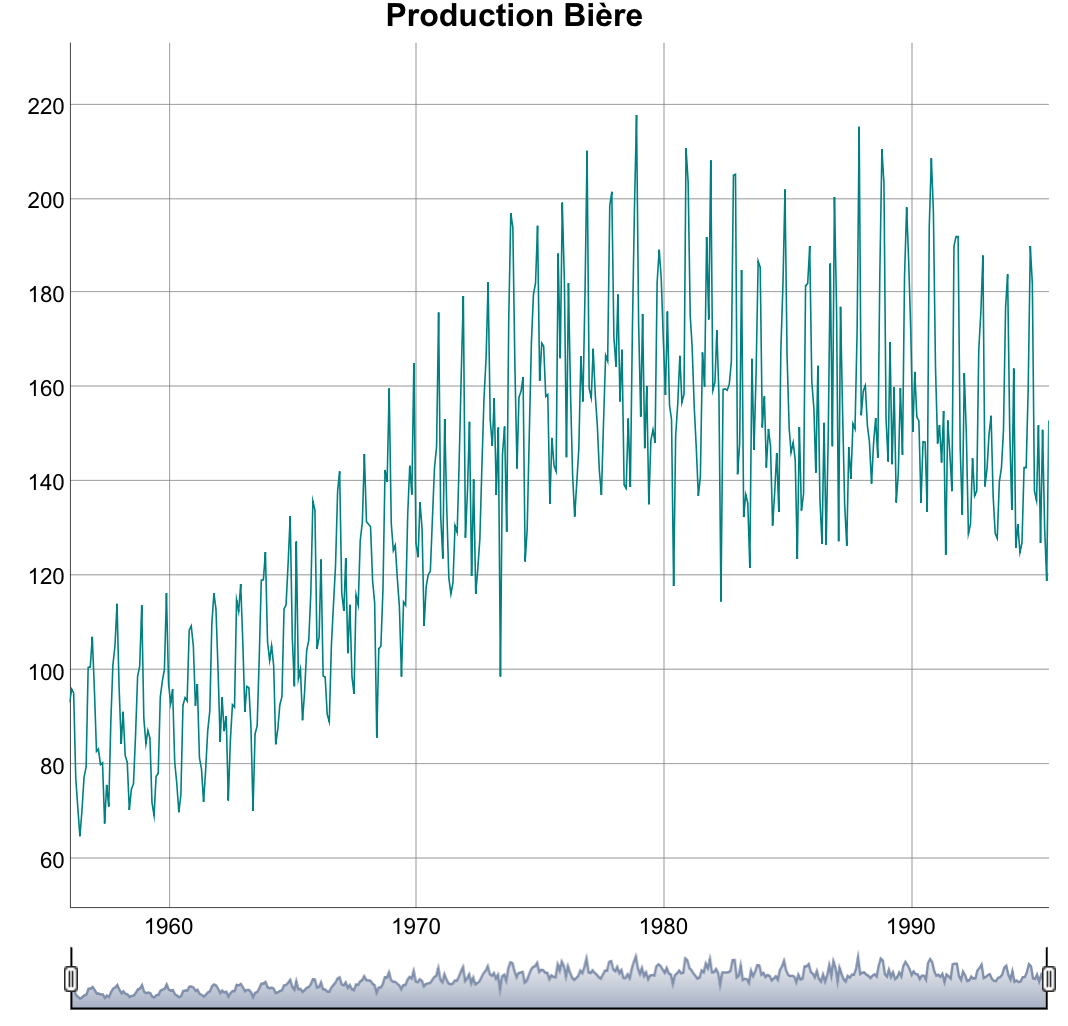
\includegraphics[width=\textwidth]{plot_beer}  
    	\caption{Série Initiale}
    	\label{fig:sub1}
    \end{subfigure}
    \begin{subfigure}{.4\textwidth}
    	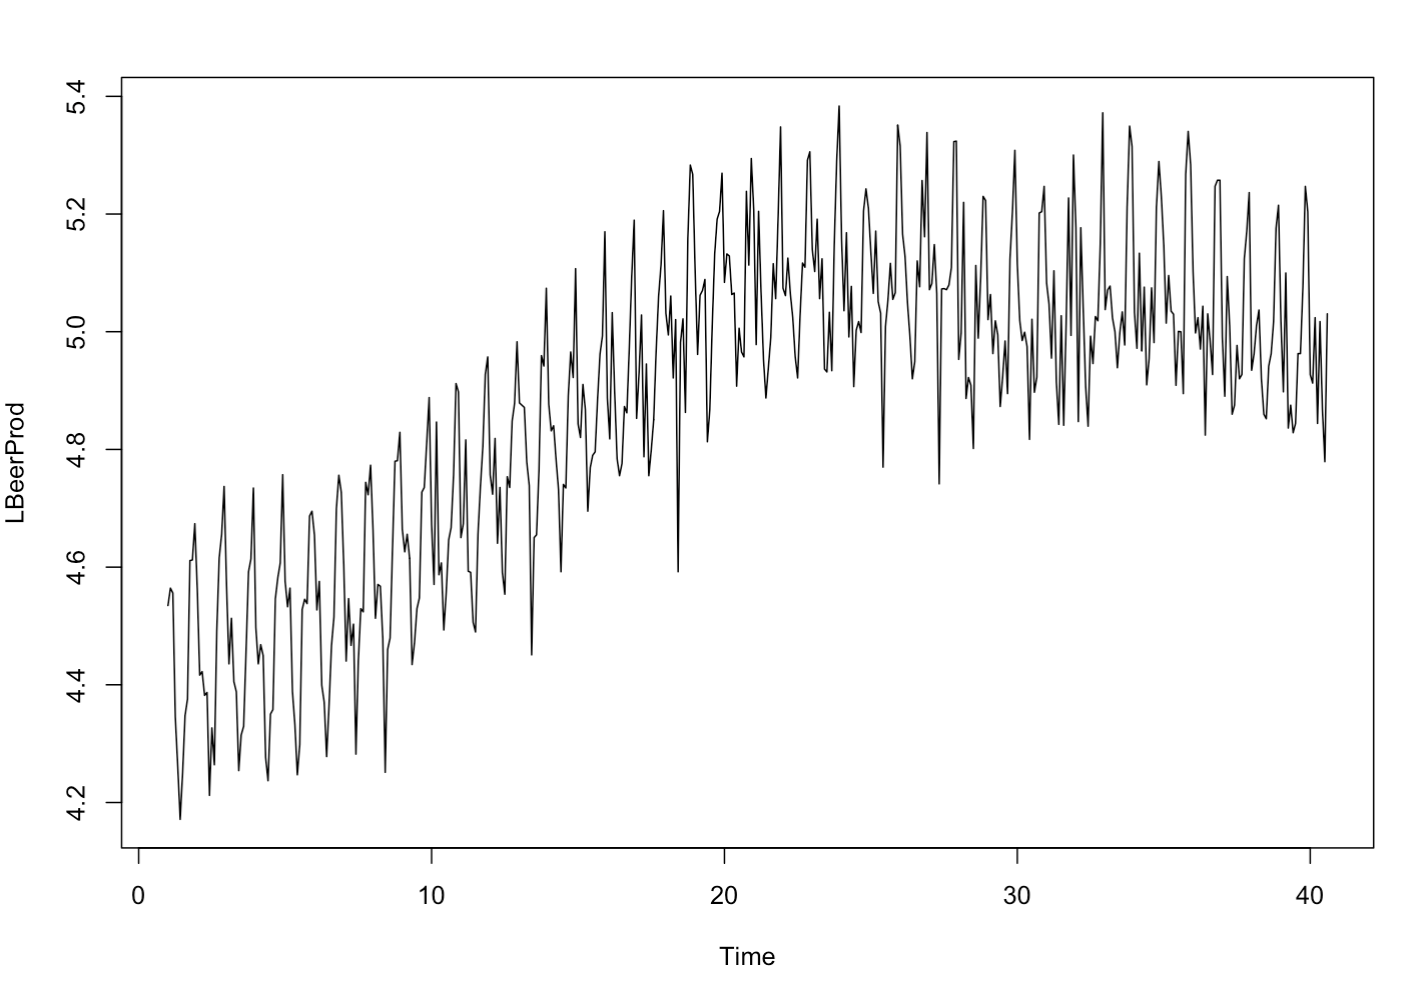
\includegraphics[width=\textwidth]{Log_Series}  
    	\caption{Série après passage au logarithme}
    	\label{fig:sub2}
    \end{subfigure}

\caption{Série initiale et série après transformation logarithmique}
\label{fig:1}
\end{figure}


\vspace{60 mm}
\subsection{Etude de la stationnarité}

\vspace{5 mm}

Nous travaillons donc maintenant en parallèle sur la série initiale et la série passée au logarithme.
La première étape pour déterminer un modèle est d'étudier la stationnarité de la série. Les tests ADF et KPSS, ainsi que l'observation visuelle des deux séries considérées montrent qu'elles ne sont clairement pas stationnaires.
Nous différencions alors plusieurs fois les séries jusqu'à obtention de la stationnarité.

Nous commençons par faire une différenciation locale sur les 2 séries (soit d=1). Les sorties ACF et PACF affichent des pics à 12, 24, et plus, nous poussant à considérer d'autres différentiations, et notamment des différentiations saisonnières (soit D=1).\\
Nous prenons ainsi les cas de différentiations suivants:
\begin{description}
  \item 1. d=0, D=1
  \item 2. d=1, D=1
\end{description}

\begin{figure}[h]
\centering
	\begin{subfigure}{.4\textwidth}
    	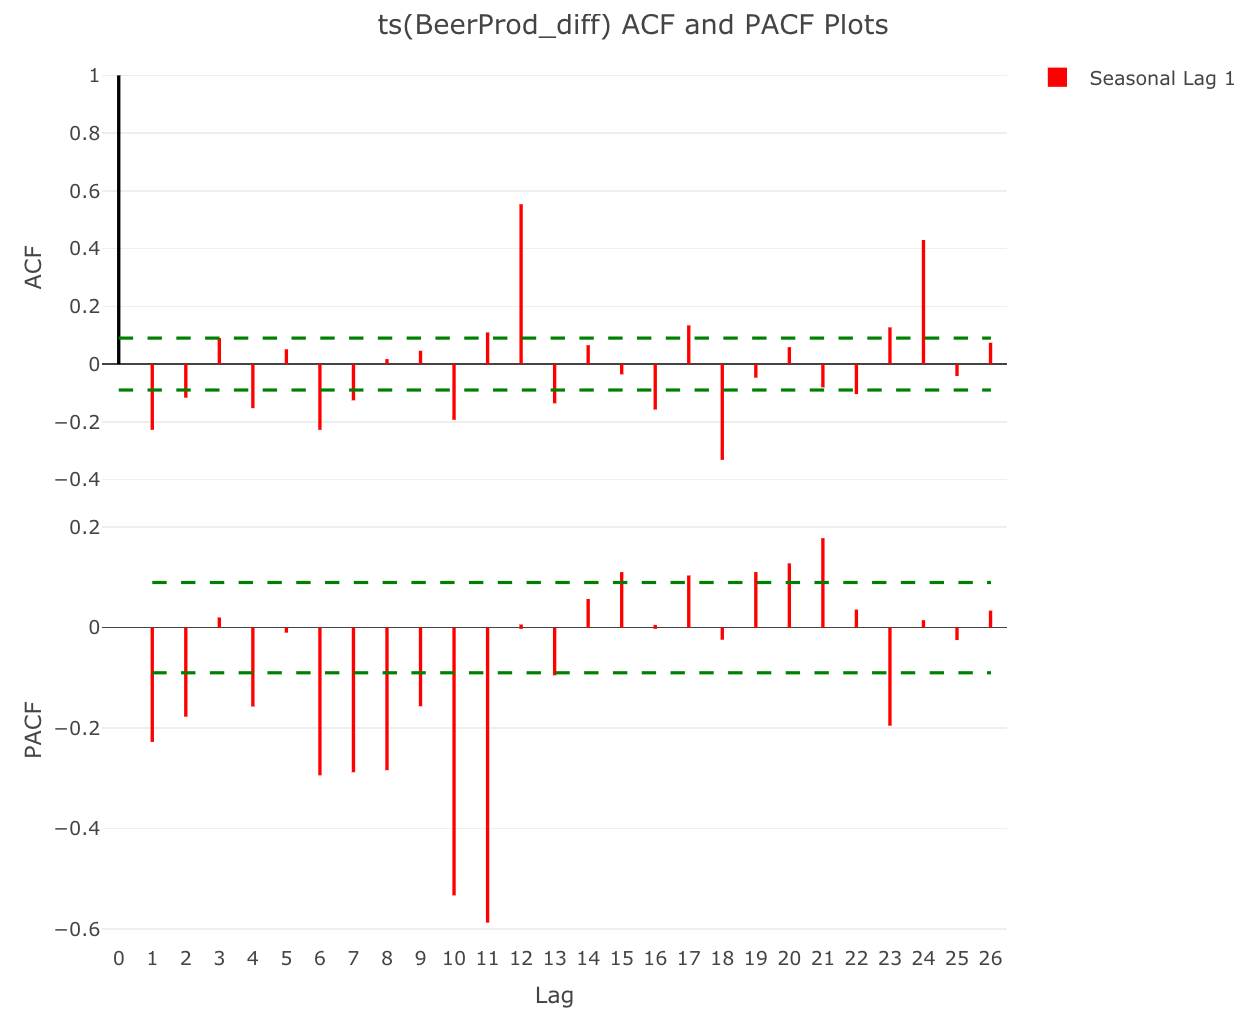
\includegraphics[width=\textwidth]{d1D0}  
    	\caption{Différentiation locale, $d=1$}
    	\label{fig:sub1}
    \end{subfigure}
    \begin{subfigure}{.4\textwidth}
    	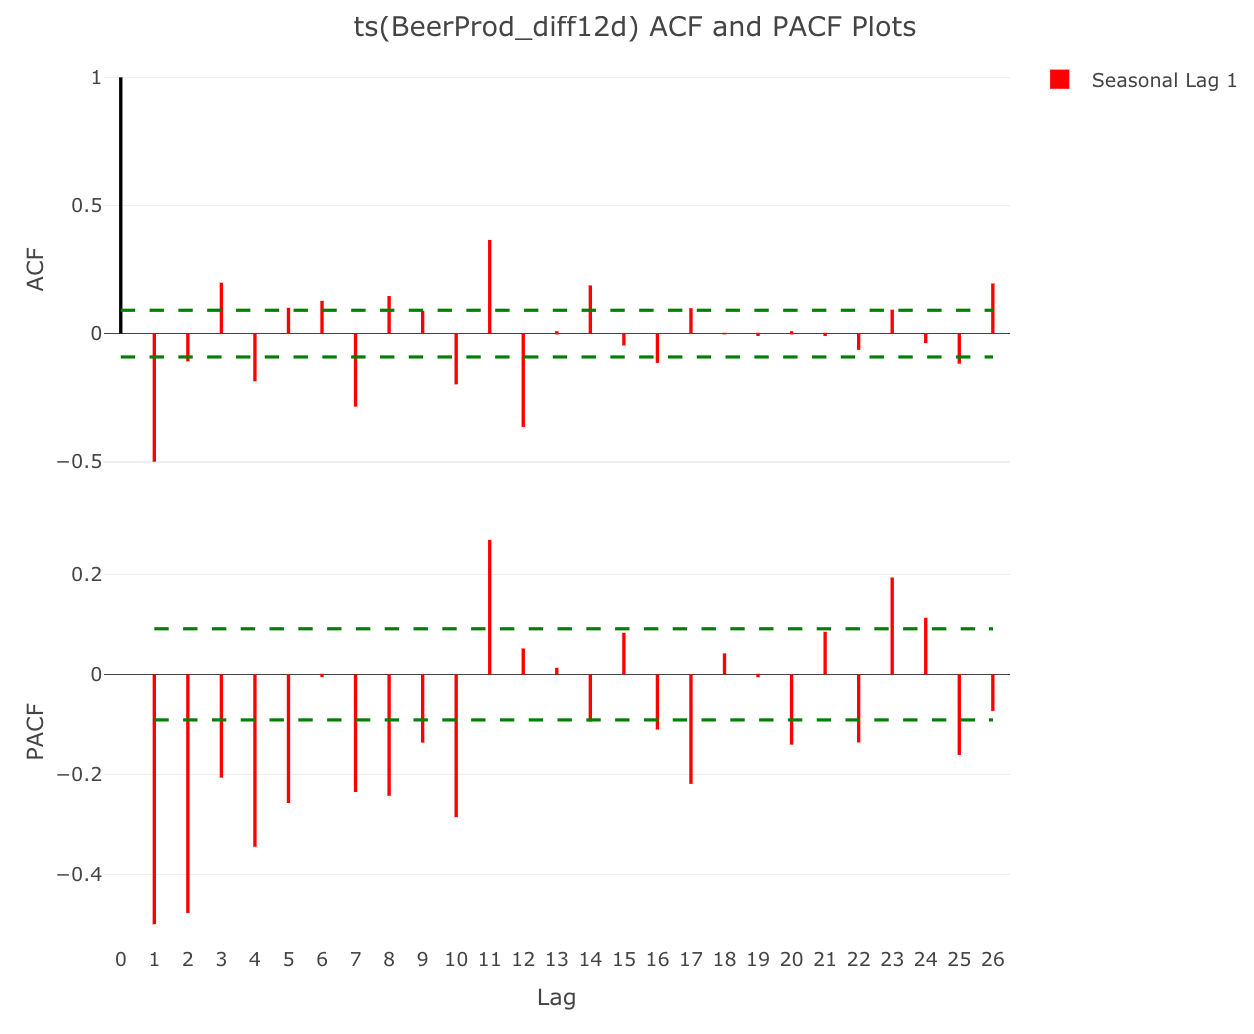
\includegraphics[width=\textwidth]{d1D1}  
    	\caption{Différentiation locale et saisonnière, $d=1, D=1$}
    	\label{fig:sub2}
    \end{subfigure}

\caption{ACF et PACF après différentiations, $d=1$}
\label{fig:2}
   
\end{figure}

\vspace{80 mm}
\noindent
Dans le premier cas, bien que les ACF et PACF ne comportent plus de pics saisonniers, la série est non-stationnaire. En revanche dans le deuxième cas : d=1,D=1, nous obtenons une série stationnaire (tests ADF et KPSS). 


\noindent 
Dans la suite on note $(X_t)_{t\in \mathbb{Z}}$ le processus initial, et $(XL_t)_{t\in \mathbb{Z}}$  le série transformée.


\vspace{5 mm}
\section{Création de modèles}

\subsection{Série Initial, $X_t$}

Nous nous focalisons en premier lieu sur la série non transformée $X_t$, puisque les approches mentionnées ci-dessous seront identiques pour la série $XL_t$.
\noindent
Nous utilisons 3 approches pour modéliser notre processus $X_t$:

\begin{figure}[h]
\centering
    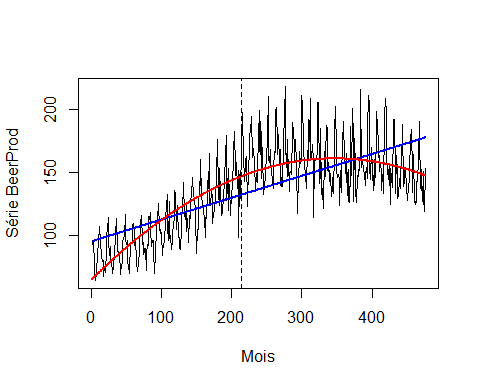
\includegraphics[scale = 0.9]{serie_tendances}  
\caption{Aperçu des différentes approches}
\end{figure}

\subsubsection{a) Première approche}
  
Dans un premier temps, nous considérons que la tendance observée sur les séries est linéaire. Nous cherchons donc grâce à la fonction auto.arima du package tseries de Rstudio les ordres p, q, P, Q optimaux, c'est à dire ceux permettant la minimisation du BIC (On impose d=1 et D=1 car ce sont ces ordres de différenciation qui éliminent la périodicité et donnent une série stationnaire).
\noindent
Nous obtenons donc un premier modèle avec p=0, q=3, P=0, Q=2. On a donc : 
$X_t \sim SARIMA(0,1,3)*(0,1,2)_{12}$
%le mettre en gras peut-être ?
\subsubsection{b) Deuxième approche}

Dans un deuxième temps, nous essayons d'affiner ce modèle en ne considérant non plus que la tendance est linéaire mais quadratique. En effet, le début de la série est bien linéaire mais à partir d'un moment, la série semble arrêter de croître pour stagner ensuite, voire décroître. \\
Pour prendre en compte cette tendance quadratique, nous décidons donc d'effectuer une régression quadratique de $X_t$ pa rapport au temps et de modéliser les résidus de cette régression par un SARIMA, toujours à l'aide de la fonction auto.arima.\\
Nous obtenons pour les résidus les ordres : p=2 d=0, q=2, P=0, D=1, P=2
  
\subsubsection{c) Troisième approche}
Enfin, au lieu de considérer que la tendance est quadratique, nous considérons qu'il y a peut-être une rupture de la tendance à un certain moment et essayons donc de repérer cet éventuel point de rupture pour diviser la série en deux et ne travailler que sur la dernière partie de la série. En effet, un évènement à pu modifier la tendance et donc prendre en compte la première partie des données risquerait de biaiser les prédictions.

\vspace{5 mm}
\noindent
Nous déterminons par étude de l'erreur MSE que le point de rupture ce trouve à l'abscisse 213 (c'est à dire en Septembre 1973). Une fois la série séparée en deux, nous ne considérons donc plus que la partie droite et modélisons cette série par un SARIMA grâce à la fonction auto.arima.\\
Nous obtenons les ordres suivant : p=0,d=0,q=0,P=1,D=1,Q=1.\\
On a donc $X2_t \sim SARIMA(0,0,0)*(1,1,1)_{12}$

\vspace{5 mm}
\begin{figure}[h]
	\begin{subfigure}{.5\textwidth}
  		\centering
    	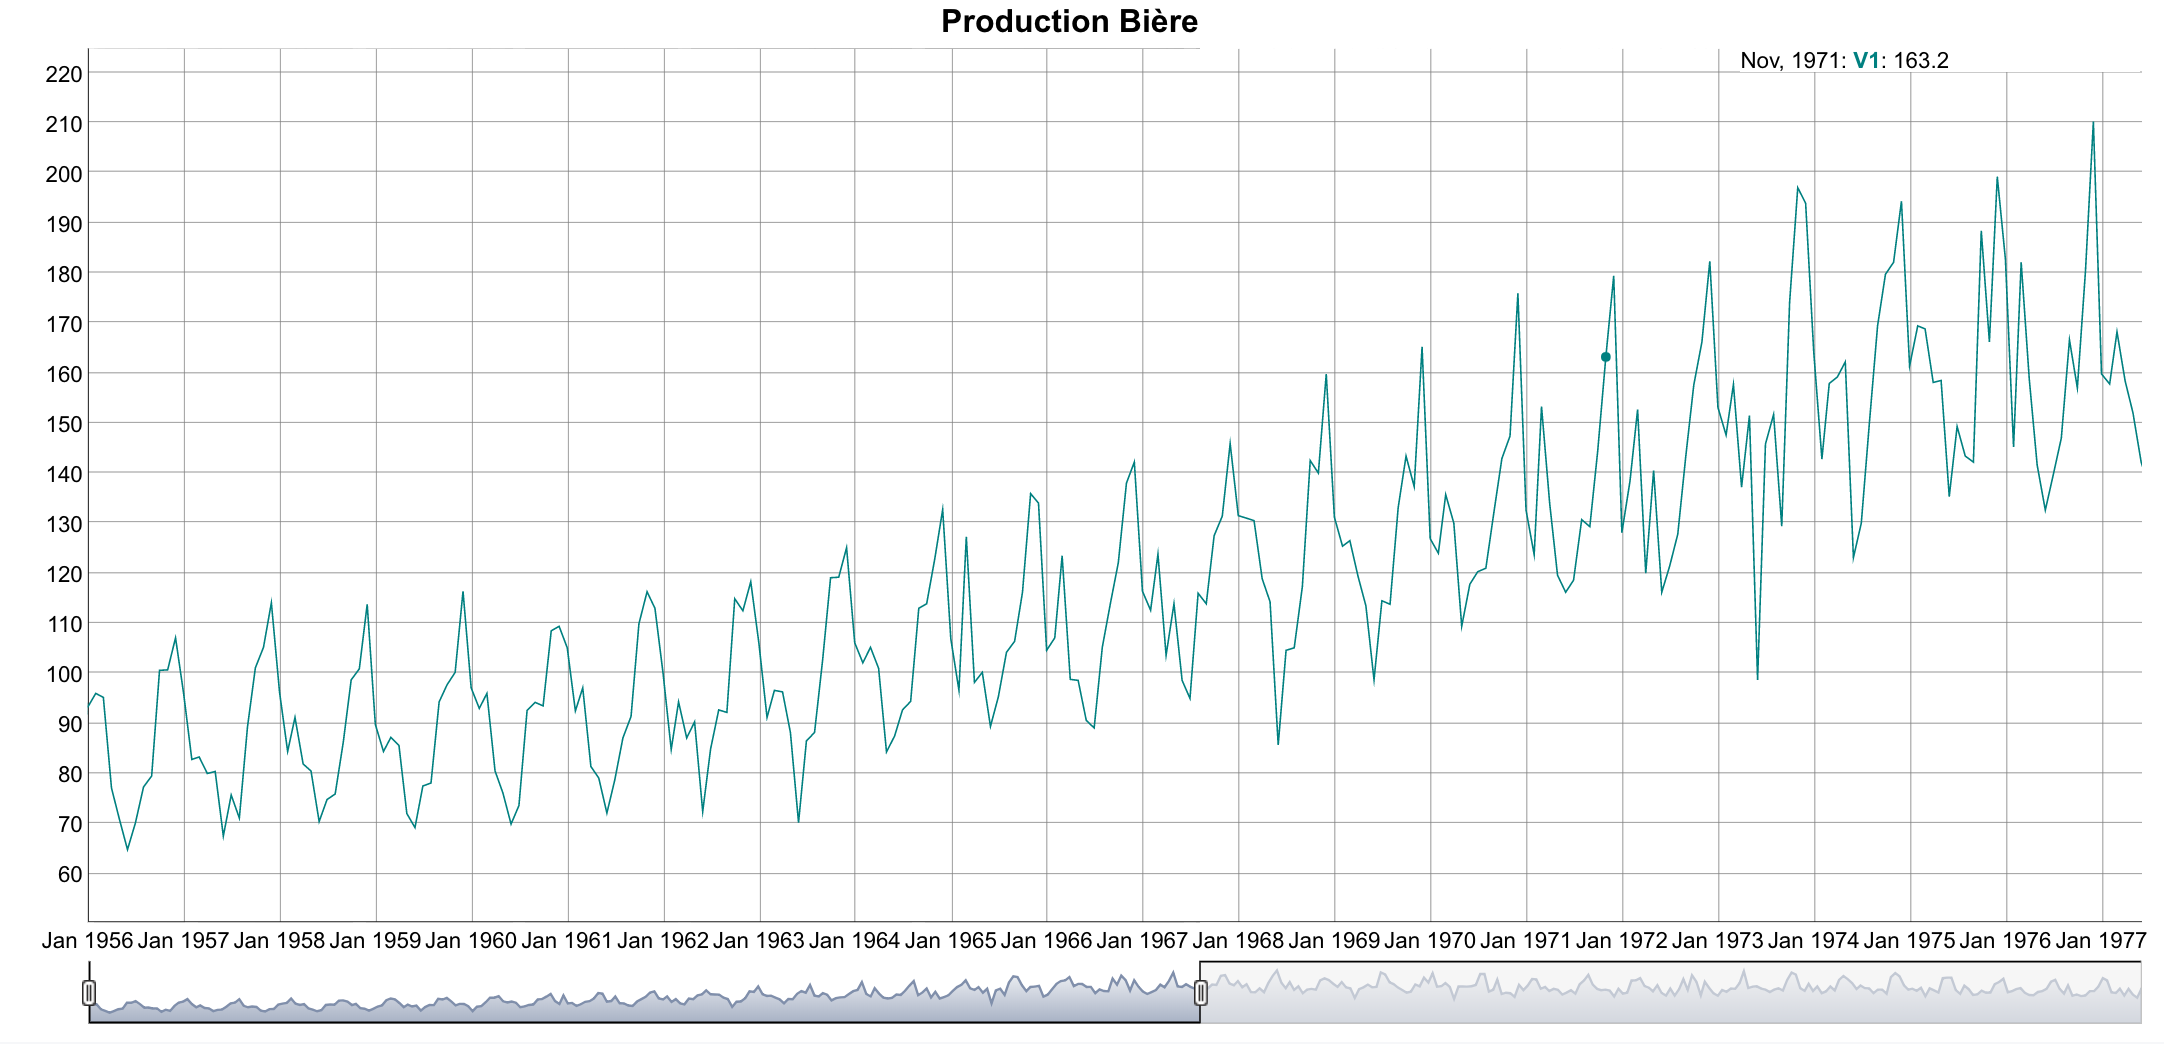
\includegraphics[width=\textwidth]{rupture1}  
    	\caption{Partie à gauche de la rupture, Série $X_1$}
    	\label{fig:sub1}
    \end{subfigure}
    \begin{subfigure}{.5\textwidth}
    	\centering
    	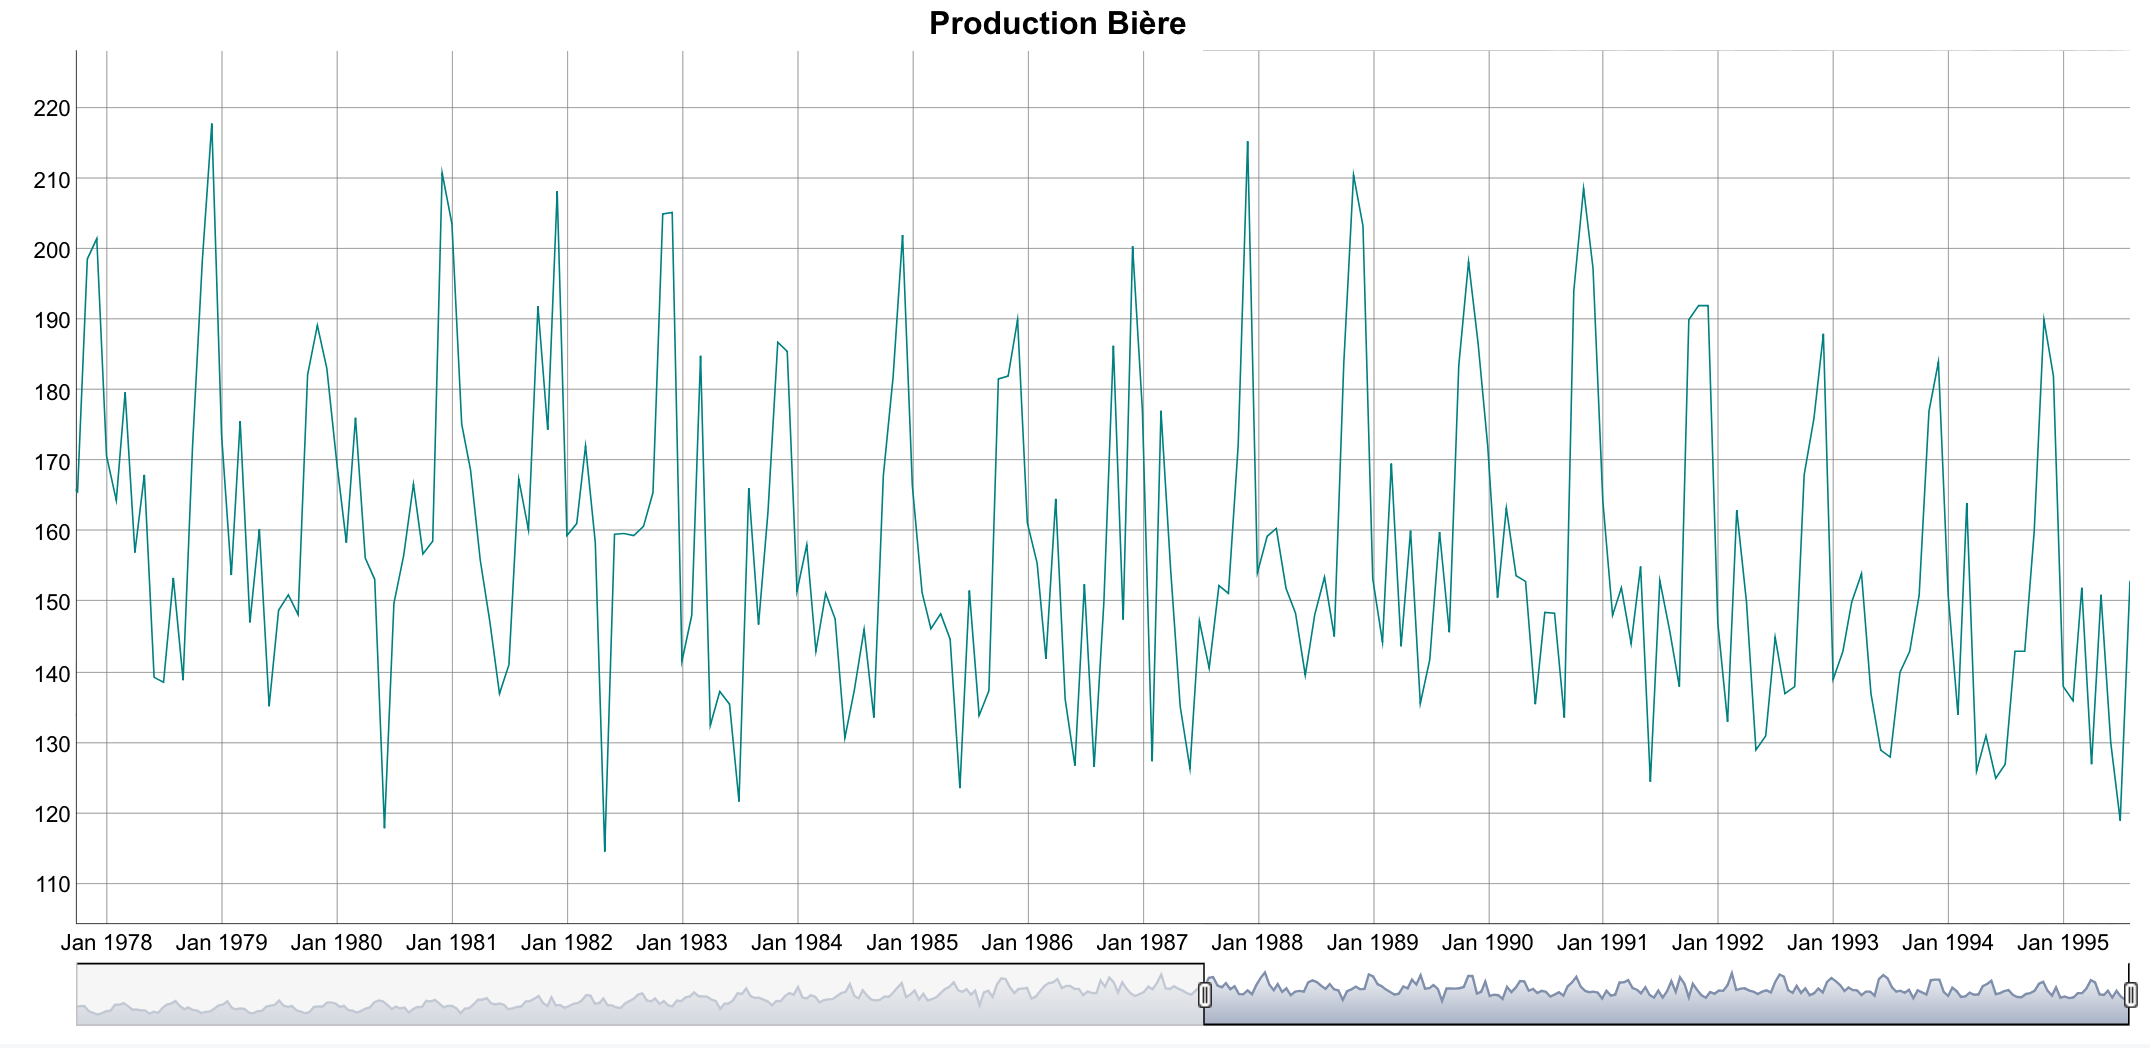
\includegraphics[width=\textwidth]{rupture2}  
    	\caption{Partie à droite de la rupture, Série $X_2$}
    	\label{fig:sub2}
    \end{subfigure}

\caption{Séparation de la série au point de rupture}
\label{fig:3}
\end{figure}

\vspace{15 mm}
Avant d'aller plus loin dans la comparaison des modèles, il est important de valider la qualité des résidus des modèles créés. Or, nous remarquons que bien que la commande auto.arima ait sélectionné les modèles minimisant le BIC, elle ne semble pas considérer la qualité des résidus. \\
En effet, le test de Box Jenkins nous montre qu'aucun des résidus ne peuvent être considérés blancs et les ACF et PACF présentent encore beaucoup de pics significatifs. Il reste donc encore beaucoup d'information à aller chercher. \\

Afin de palier à ce problème nous cherchons alors à augmenter manuellement les valeurs de p, q ainsi P et Q au risque d'avoir des paramètres non significatifs. Une fois ces valeurs augmentées ou diminuées, nous regardons la significativité de chaque estimateur. Si un estimateur n'est pas significatif , nous l'enlevons du modèle et comparons les valeurs du BIC pour les modèles avec et sans. Nous gardons enfin le modèle qui minimise le BIC.

\begin{figure}[h]
\centering
    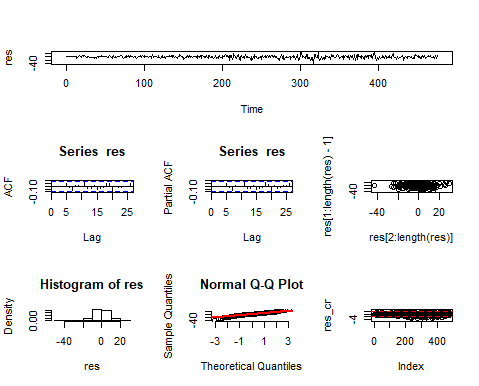
\includegraphics[width=\textwidth]{beaux_residus}  
\caption{Checkup des résidus obtenus après modifications des ordres}
\end{figure}

\noindent
Nous obtenons donc finalement les modèles 'optimaux' suivants:

\begin{table}[h]
  \begin{center}
    \caption{Modèles retenus}
    \label{tab:table1}
    \begin{tabular}{l|c}
      \ & \textbf{Modèles}\\
      \hline
      Mod1 & SARIMA $(4,1,4)(0,1,1)_{12}$\\
      Mod2 & SARIMA $(4,0,4)(0,1,1)_{12}$ (sur les résidus)\\
      Mod3 & SARIMA  $(4,1,3)(0,1,1)_{12}$ (rupture)\\
    \end{tabular}
  \end{center}
\end{table}

\vspace{20 mm}
\subsection{Série avec transformation logarithmique, $XL_t$}

Nous procédons de la même façon avec le modèle logarithmique.Nous obtenons par les 3 mêmes approches et après ajustement des paramètres les modèles suivants : 

\begin{table}[h!]
  \begin{center}
    \caption{Modèles retenus}
    \label{tab:table1}
    \begin{tabular}{l|c}
      \ & \textbf{Modèles}\\
      \hline
      ModL1 & SARIMA $(3,1,4)(0,1,1)_{12}$\\
      ModL2& SARIMA $(4,0,4)(0,1,1)_{12}$ (sur les résidus)\\
      ModL3 & SARIMA $(4,0,4)(0,1,1)_{12}$ (rupture)\\
    \end{tabular}
  \end{center}
\end{table}

\vspace{5 mm}
\section{Comparaison des modèles et prédictions}

\subsection{Meilleurs modèles}

Pour chaque série, nous comparons les 3 modèles obtenus sur la base d'un critère prédictif. Nous prédisons à nouveau la dernière période de la série à l'aide des modèles tronqués et calculons l'erreur MSE pour chaque modèle (carré des écarts). Nous gardons le modèle qui minimise la MSE.\\
Les modèles retenues (Tables 3 et 4) sont donc les suivants : 

\noindent
\textbf{Série $X_t$ : Modèle 2: SARIMA$(4,0,4)(0,1,1)_{12}$}

\begin{table}[h!]
  \begin{center}
    \caption{MSE à partir de la série initiale}
    \label{tab:table1}
    \begin{tabular}{l|c|r} 
      \ & \textbf{Modèles} & \textbf{MSE}\\
      \hline
      1 & SARIMA $(4,1,4)(0,1,1)_{12}$ & 69.82345\\
      \rowcolor{LightCyan}
      2 & SARIMA $(4,0,4)(0,1,1)_{12}$ (sur les résidus)& \textbf{66.83503}\\
      3 & SARIMA $(4,1,3)(0,1,1)_{12}$ (rupture) & 77.87975\\
    \end{tabular}
  \end{center}
\end{table}

\noindent
\textbf{Série $XL_t$ : Modèle L3 : SARIMA$(4,0,4)(0,1,1)_{12}$}

\begin{table}[h!]
  \begin{center}
    \caption{MSE à partir de la série transformée}
    \label{tab:table1}
    \begin{tabular}{l|c|r} 
      \ & \textbf{Modèles} & \textbf{MSE}\\
      \hline
      L1 & SARIMA $(3,1,4)(0,1,1)_{12}$ & 0.003685328\\
      L2 & SARIMA $(4,0,4)(0,1,1)_{12}$ (sur les résidus)& 0.003874816\\
      \rowcolor{LightCyan}
      L3 & SARIMA $(4,0,4)(0,1,1)_{12}$ (rupture)& \textbf{0.003226944}\\
    \end{tabular}
  \end{center}
\end{table}

\vspace{5 mm}
\subsection{Prédictions}

Une fois le meilleur modèle déterminé pour chaque séries, nous passons à l'étape de prédiction.\\
Les graphiques ci-dessous montrent les prédictions des deux modèles retenus, sur 3 ans. À gauche, la prédiction du modèle 2, à droite celle du modèle L3. Le dernier graphique représente les intervalles de prédiction de ces deux modèles.

\begin{figure}[h!]
	\begin{subfigure}{.5\textwidth}
  		\centering
    	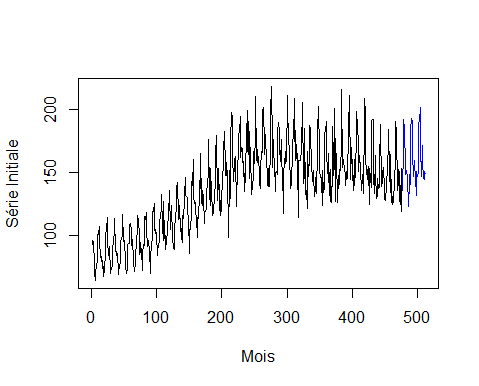
\includegraphics[width=\textwidth]{pred_mod2}  
    	\caption{Prédiction avec le Modèle 2}
    	\label{fig:sub1}
    \end{subfigure}
    \begin{subfigure}{.5\textwidth}
    	\centering
    	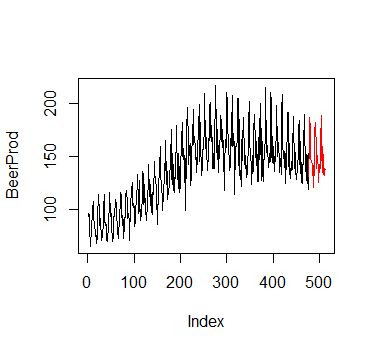
\includegraphics[width=\textwidth]{pred_modL3}  
    	\caption{Prédiction avec le Modèle L3}
    	\label{fig:sub2}
    \end{subfigure}

\caption{Prédictions sur 3 ans}
\end{figure}

\begin{figure}[h!]
    \centering
    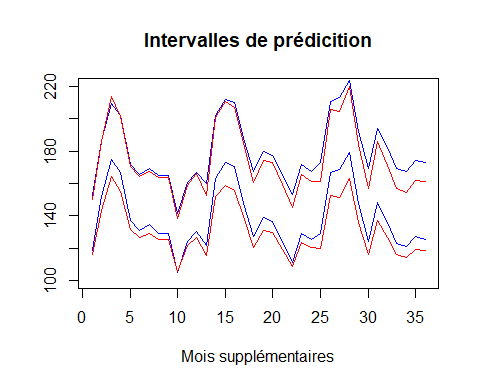
\includegraphics[scale=0.7]{int_pred}  
    \caption{Intervalles de prédiction des deux modèles}
\end{figure}


\vspace{30 mm}

\noindent
{\LARGE \textbf{Conclusion}}

\vspace{5 mm}
Après une rapide étude visuelle de la série, nous avons pu déterminer trois différentes approches pour la modélisation de celle-ci. Dans chaque approche, nous étudions plus en détails les ACF et PACF des différentes différenciations effectuées. Nous étudions également la blancheur des résidus et la significativité des estimateurs des modèles renvoyés par la fonction auto.arima. Nous obtenons ainsi 6 modèles que nous comparons 3 à 3 sur un critère prédictif. Les erreurs MSE associées à chaque modèles nous permettent de déterminer un modèle optimal pour la série initiale et la série transformée. Nous prédisons ainsi avec ces deux modèles la production de bière en Australie pour les 3 années suivantes. 
Après étude des intervalles de prédiction nous serions tentées de dire que le modèle 2 est meilleure que le modèle L3 car ces intervalles sont plus petits, donc la prédiction est plus 'sûre' que celle du modèle L3. Cependant, cela reste assez ambigüe et il donc très difficile de dire quel modèle est meilleur dans cette situation.

\end{document}